% last updated in April 2002 by Antje Endemann
% Based on CVPR 07 and LNCS, with modifications by DAF, AZ and elle, 2008 and AA, 2010, and CC, 2011; TT, 2014; AAS, 2016

\documentclass[runningheads]{llncs}
\usepackage{graphicx}
\usepackage{amsmath,amssymb} % define this before the line numbering.
\usepackage{ruler}
\usepackage{color}\usepackage{array}
\usepackage{cite}

\usepackage{caption} 
\captionsetup[table]{skip=3pt}

\newcommand{\etal}{\mbox{\emph{et al.\ }}}

\usepackage[width=122mm,left=12mm,paperwidth=146mm,height=193mm,top=12mm,paperheight=217mm]{geometry}

\makeatletter
\newcommand{\thickhline}{%
    \noalign {\ifnum 0=`}\fi \hrule height 1pt
    \futurelet \reserved@a \@xhline
}

\makeatletter
\renewcommand\paragraph{\@startsection{paragraph}{4}{\z@}%
           {1.25ex \@plus1ex \@minus.2ex}%
           {-1em}%
           {\normalfont\normalsize\bfseries}}
            
\renewcommand\subsubsection{\@startsection{subsubsection}{3}{\z@}%
                {-2ex\@plus -1ex \@minus -.2ex}%
                {0.1ex \@plus .2ex}%
                {\normalfont\normalsize\bfseries}}
                
                
\newcolumntype{"}{@{\hskip\tabcolsep\vrule width 1pt\hskip\tabcolsep}}
\makeatother\begin{document}
% \renewcommand\thelinenumber{\color[rgb]{0.2,0.5,0.8}\normalfont\sffamily\scriptsize\arabic{linenumber}\color[rgb]{0,0,0}}
% \renewcommand\makeLineNumber {\hss\thelinenumber\ \hspace{6mm} \rlap{\hskip\textwidth\ \hspace{6.5mm}\thelinenumber}}
% \linenumbers
\pagestyle{headings}
\mainmatter
\def\ECCV16SubNumber{1644}  % Insert your submission number here

\title{Joint Event Recognition and Image Curation} % Replace with your title

\titlerunning{ECCV-16 submission ID \ECCV16SubNumber}

\authorrunning{ECCV-16 submission ID \ECCV16SubNumber}

\author{Anonymous ECCV submission}
\institute{Paper ID \ECCV16SubNumber}


\maketitle

\begin{abstract}
Automatic image organization of personal photos is a problem with many real world applications, and can be divided into two main tasks: recognizing event types of the photo collections, and selecting interesting images from the collections. The two tasks are both challenging, in that the photos from the same event type are highly varied, and there is a great deal of overlap in photos from different event types. In this paper, we looked into the possibility of simultaneously solving both tasks: album-wise event recognition and image-wise importance prediction conditioned on the recognized event types. We collected an event album dataset with both event type labels and image importance labels, refined from the existing CUFED dataset. We propose a hybrid system consisting of three parts: Siamese network based event-specific image importance prediction, Convolutional Neural Network(CNN) based event recognition, and Long Short-Term Memory(LSTM) based sequence level event recognition, and we propose an iterative updating procedure for event type and image importance score prediction. We show with experiments that the proposed method outperforms the classical approach based on single static image classification, and more importantly, we verified that image importance score prediction and event type recognition can in turn help the performance of each other. 


\keywords{Event Recognition, Image Importance, Convolutional Neural Network, Long Short-Term Memory}
\end{abstract}


\section{Introduction}
With the advent of cheap cameras in nearly all of our devices,  automated uploading to the cloud, and practically unlimited storage,
%With the rapid progress in portable photo taking devices and the increasing volume of storage devices and services,
it becomes painless to take photos frequently in daily life, resulting in the explosion of personal photo collections. However, the oversized image collections make it difficult to organize the photos, and thus automatic organization algorithms are highly desirable. The organization of personal photo collections can be decomposed into two stages: recognizing the event type of a photo collection, and suggesting the most interesting/important images in the photo collection to represent the album. This can be used to pick photos for an album cover, and to make a photo book. The two stages assist users in keeping the photo collections organized and free of irrelevant images.

Both event recognition and image importance prediction have been studied independently in previous literature. Studies of event recognition can be categorized into several types. The most popular branches of study use videos as input \cite{2015trecvidover, TangCVPR12, xu2015discriminative}, so spatiotemporal feastures are used for the task. 
At the other end of the spectrum, event recognition for single images has also been attempted \cite{what_where, Park_2015_CVPR_Workshops, cSalvadora}. In contrast to video-based event recognition, there is no temporal information to exploit, and there is no need to consider relevant frame importance or contribution to the event, since there is only one ``frame." This problem can be viewed as a special case of scene recognition, and both object level features and scene level features are used \cite{what_where}. 

Album-wise event recognition lies in the middle between single-image-based and video-based event recognition, and is the most related branch to our work. Images in an album can be thought of as very sparse samples from the event video. Photo albums differ from videos in that consecutive images from the photo album are no longer continuous, and can have very different visual and semantic information. However, there is still sequential information in time-stamped albums. In \cite{HMM}, the success of an HMM-based model for album event recognition indicates that the sequential information in an album is still very helpful for  album-wise event recognition.

Image importance is a complex image property which is related to various factors, such as aesthetics \cite{aesthe_14}, interestingness \cite{interesting} and image memorability \cite{Isola2011}. It has been shown \cite{CVPR} that image importance is modulated by the context of the image, i.e., image importance is album-dependent, or event-specific. Event-specific image importance is a highly subjective judgment, and learning it is a very challenging task, due to the very high intra-class variability, and the underlying uncertainty caused by the subjectiveness of the property. Nevertheless, recent work \cite{CVPR} based on Convolutional Neural Networks (CNNs) shows that it can be reasonably predicted. 

Event recognition and image importance prediction are inherently related to one other: 1) importance prediction is event-dependent, so we need to know the event to better predict importance; 2) albums often contain 		``outlier" photos that aren't directly related to the event, which affects event prediction. So if we know the important/key images in an album, we better recognize the event type.  Therefore, returning to the task of photo collection organization, we ask the question: can we simultaneously recognize the event type for an album, and discover important images in the event album? 

To answer this question, this paper makes the following contributions: 1) We develop a joint event recognition and image importance prediction algorithm, which has not been addressed before. We use a CNN for image level event recognition, and a Siamese Network for event-specific image importance prediction. An iterative update scheme is conducted during the test stage, and we find that event recognition and image importance prediction can improve each other's performance; 2) We further boost the performance of event recognition with an LSTM network that leverages sequence information in labeling the album; 3) We also refine the CUFED dataset by collecting more human annotations for the event types, allowing raters to apply multiple labels to the events. This improves the reliability of the ground-truth, making explicit the ambiguity between event types. This provides us with more training information, and allows for a fairer evaluation at the testing stage.

\section{Related Work}


Our work is partly inspired by \cite{CVPR}, who proposed a novel image property: event-specific image importance. In that work, it was claimed that image importance or ``interestingness" is contextual and is related to the album it is in. For example, a photo of a beautiful work of architecture is important in an album of an urban trip, yet not so important in a wedding event.  A Siamese network is used to predict the relative importance score difference between an input image pair, and is jointly trained on all event types.

However, in \cite{CVPR}, it is assumed that the event type of the album is already known. This is unacceptable if we want to build an end-to-end photo organization algorithm. In this work, we relax this assumption and train a system simultaneously for event recognition and image curation, so that additional user input of the event type is not required.


Our work is also closely related to the study of event recognition for a personal album. The model in \cite{Mattivi11} classifies a personal album into 8 social events and 10 sports events simply by aggregating SVM classification results from single images in the album. In \cite{pattern}, Tsai \etal exploit object level patterns for event type recognition. Object patterns are learnt from single images,  and then an album-wise SVM is trained on the frequency distribution of different object patterns appearing in an album. Similarly, Imran \etal \cite{Imran09} use the Pagerank technique to mine the most useful features for an event, and an album-wise SVM classifier is used for recognition.
% * <gary@ucsd.edu> 2016-03-15T03:31:47.272Z:
%
% > Pagerank technique to mine the most useful features
%
% I have a hard time understanding how the pagerank technique could be applied here. Can you be more specific?
%
% ^.
% * <gary@ucsd.edu> 2016-03-15T03:30:37.974Z:
%
% > Object patterns
%
% What is an "object pattern"? Clarify with an example.
%
% ^.
The above work treats albums as unordered collections of images. On the other hand, in \cite{HMM}, Bossard \etal exploit the sequential nature of personal albums and use an HMM based sub-event approach for event recognition. They use temporal sequence of the images, and model an album with successive latent sub-events to boost the recognition performance. It has been shown that the temporally-sensitive HMM outperforms the simple aggregation of predictions from all the images in an album.  They also collected a 14 class dataset consisting of 807 albums for the task as a benchmark for album-wise event recognition. 
% * <gary@ucsd.edu> 2016-03-15T03:33:18.445Z:
%
% > It has been shown
%
% They show? Instead of "it has been shown"? Did they show this? If so, say "They show"
%
% ^.


Event recognition for single photos has also been studied.  Li \etal \cite{what_where} use a generative graphical model to recognize event types of a database with 8 sports events. Their model integrates cues from scene and object categorization to classify the sports events. Deep Neural Networks, especially  Convolutional Neural Networks(CNNs) provide us with outstanding visual representations that can be used for the single static image event recognition task\cite{Park_2015_CVPR_Workshops, cSalvadora}. Salvador \etal\cite{cSalvadora} apply CNNs to cultural event recognition. They integrate cues from visual features extracted by a CNN with the time-stamp of a photo, inspired by the fact that photos of a cultural event are mostly taken in the same period of time. However, in personal photo collections, the relevance of an image within an event album varies a great deal. These approaches for single images are useful, but not sufficient for album-wise event recognition.
% * <gary@ucsd.edu> 2016-03-15T03:37:09.346Z:
%
% > However, in personal photo collections, the relevance of an image within an event album varies a great deal. These approaches for single images are useful, but not sufficient for album-wise event recognition.
%
% I'm not sure these two sentences go together. The first is about image importance, and the second is about event recognition. Are you trying to make two points, or one?
%
% ^.
% * <gary@ucsd.edu> 2016-03-15T03:34:56.897Z:
%
% > cultural event recognition
%
% What kind of "cultural events"? Do you mean events that occur at the same time each year, like the 4th of July, Christmas, and New Year's Eve? Mention that, otherwise "cultural events" is a bit of an obscure designation.
%
% ^.

Convolutional Neural Network(CNN) methods have greatly boosted performance in image understanding tasks, such as image classification, object detection and scene recognition \cite{imagenet, googlenet, rcnn, places}. Now a many researchers have switched their focus to higher-level image properties, such as event recognition \cite{event_recognition}, semantic segmentation \cite{long_shelhamer_fcn},  multilabel image annotation \cite{tagging}, and image captioning \cite{lrcn}. 

Long Short-Term Memory(LSTM) networks \cite{lstm} have been proposed for sequence prediction and sequence labeling. LSTM networks have advantages over traditional Recurrent Neural Networks (RNN) in that they can maintain contextual information across  an extended sequence of inputs. LSTMs have achieved success for tasks such as handwritten text recognition \cite{Graves} and speech recognition \cite{speech}. 
The success of LSTMs for sequence prediction tasks have also been extended to video-based event recognition. In \cite{lstm}, the LSTM network and visual feature extraction network is stacked, and the network can deal with both event recognition and description. Reiter \etal \cite{lstm2} also combine LSTM and HMMs for video meeting analysis. Relevant to our work, the Long-term Recurrent Convolutional Network (LRCN) model \cite{lrcn} has been proposed to stack CNN feature extractors and LSTM networks for sequential learning of videos or images.


\section{The ML-CUFED Dataset}
In order to train and evaluate the joint curation-recognition model, we use the Curation of Flickr Events Dataset (CUFED) \cite{CVPR}, and refine it by collecting more human opinions on the event types in the dataset. We call the new dataset MultiLabel-CUFED (ML-CUFED). In this section, we describe the dataset, and provide a consistency analysis of the labels collected from Amazon Mechanical Turk (AMT). The dataset will be made available to the public.
\subsection{The CUFED Dataset}
The CUFED Dataset \cite{CVPR} is an image curation dataset extracted from the Yahoo Flickr Creative Commons 100M Dataset (YFCC100M).  It contains 1883 albums over 23 common event types from our daily life, ranging from 50 to 200 albums for each event type. The event type of each album was decided by three workers' annotations through Amazon Mechanical Turk (AMT). Meanwhile, within each album, the event-specific importance score of each image is obtained by averaging 5 AMT workers' votes when the event type is given to them. 

One problem the CUFED Dataset has is that the event type of an album is decided by only three workers, who were constrained to give a single label to each album. However, some of the event types identified in that dataset are related (e.g., architecture and urban trip). For an album with ambiguous event types or with multiple event types, such a constraint is overly restrictive. For example, the two albums in Fig~\ref{album} are both birthday events, but they can also fall into the category of casual family/friends gathering. These two event types are not mutually exclusive. Moreover, intuitively, we would consider the album on the right to be a more typical birthday event, with distinguishable elements such as birthday hats and cakes, while the album on the left is more of a casual family/friends gathering rather than an obvious birthday event. Therefore, collecting the event types and their proportion in one album from more peoples' views is necessary. This results in a multi-label event recognition dataset with richer information. 
% * <gary@ucsd.edu> 2016-03-15T03:54:37.133Z:
%
% > while the album on the left is more of a casual family/friends gathering rather than an obvious birthday event.
%
% does it contain any images of a cake? If not, say so!
%
% ^.
\begin{figure}
\centering
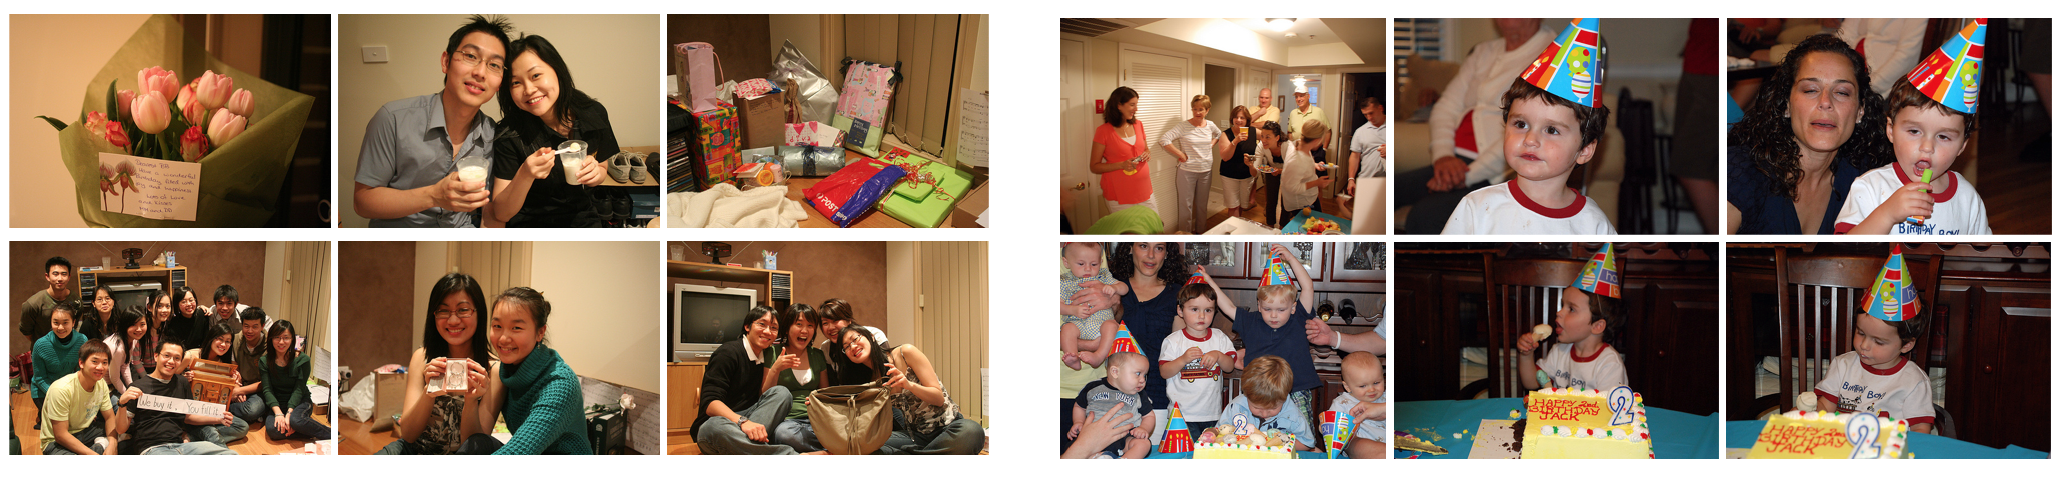
\includegraphics[width=4.5in]{album}
\caption{Example of two birthday albums (both have the photo uploader's tag ``birthday"). }
\label{album}
\vspace{-0.15in}
\end{figure}




\subsection{Data collection}
In addition to the three votes the dataset already includes, we collected 9 more workers' opinions, and allowed for multiple choices for each album. We allowed workers to select up to three event types for an album. There were  299 distinct workers who participated in the task.

Quality control was performed for each AMT worker in order to collect high quality annotations. Before the real task, only workers who passed an album event recognition test (which is very similar to the actual task) were allowed to proceed to work on the actual task. During the tasks, there was another round of quality control. After workers submitted the tasks, the results they turned in were compared with other workers' submissions, and submissions that highly diverged from others were further manually inspected. If the divergence was unreasonable, the submission was rejected. After all the annotations from workers were collected, we further cleaned the annotations by eliminating the labels with very rare votes: for each album, all the event types with only one vote were discarded. 
% * <gary@ucsd.edu> 2016-03-15T03:57:28.489Z:
%
% > for each album, all the event types with only one vote were discarded. 
%
% How many of these votes were discarded?
%
% ^.
% * <gary@ucsd.edu> 2016-03-15T03:57:00.649Z:
%
% > If the divergence was unreasonable, the submission was rejected.
%
% how many submissions were rejected in this way?
%
% ^.

For the final ground-truth event types and their proportion of one album, we use the the proportion of votes among all the votes. For workers who give votes to more than one label, each of their votes is normalized so that all the votes sum to one.
% * <gary@ucsd.edu> 2016-03-15T03:58:28.356Z:
%
% >  we use the the proportion of votes among all the votes.
%
% Perhaps: "We converted the votes to a probability distribution over event types."
%
% ^.

\subsection{Dataset Analysis}
To check the validity of the dataset we collected, we analyzed the annotations in several ways. Each album has between 9 and 27 votes (because we allow for multiple choices from one worker). 76\% of the albums received votes for two or fewer event types. This suggests the high coherence of those albums. 95\% of the albums received votes for three or fewer event types.  To check the consistency among workers, we randomly split the 299 workers into two halves, and for each album we checked whether the annotations from one half was consistent with the other half. For each album, we examined whether the top event types suggested by these two independent groups were the same.
% * <gary@ucsd.edu> 2016-03-15T03:59:52.326Z:
%
% > 95\% of the albums received votes for three or fewer event types. 
%
% I don't understand: Don't 100% of the albums receive 3 or fewer event type votes?
%
% ^.
We repeated the random split 100 times, and on average, for 89.6\% of the albums, the event type receiving most votes were the same for both groups. This suggests that despite the ambiguity of some album types, the opinions of different AMT workers were consistent.

\section{Joint Event Recognition and Image Curation}
\label{approach}
In this section, we describe our approach to jointly attain image importance prediction and album event-type recognition. It is intuitive that important images contribute  more to the identity of an event, and should be emphasized when deciding the event type of the album from the images. Also, the identity of event is needed for accurate individual image importance prediction, as shown in \cite{CVPR}. Moreover, it has been shown that sequential information in an album is useful for the prediction. Therefore, we build a joint system that can simultaneously predict the event type and image importance ratings for an album. The system is shown in Figure~\ref{figure1}. We  elaborate on the different parts of the system in the rest of this section.
% * <gary@ucsd.edu> 2016-03-15T04:04:56.901Z:
%
% > Moreover, it has been shown that sequential information in an album is useful for the prediction.
%
% reference?
%
% ^.

\begin{figure}
\centering
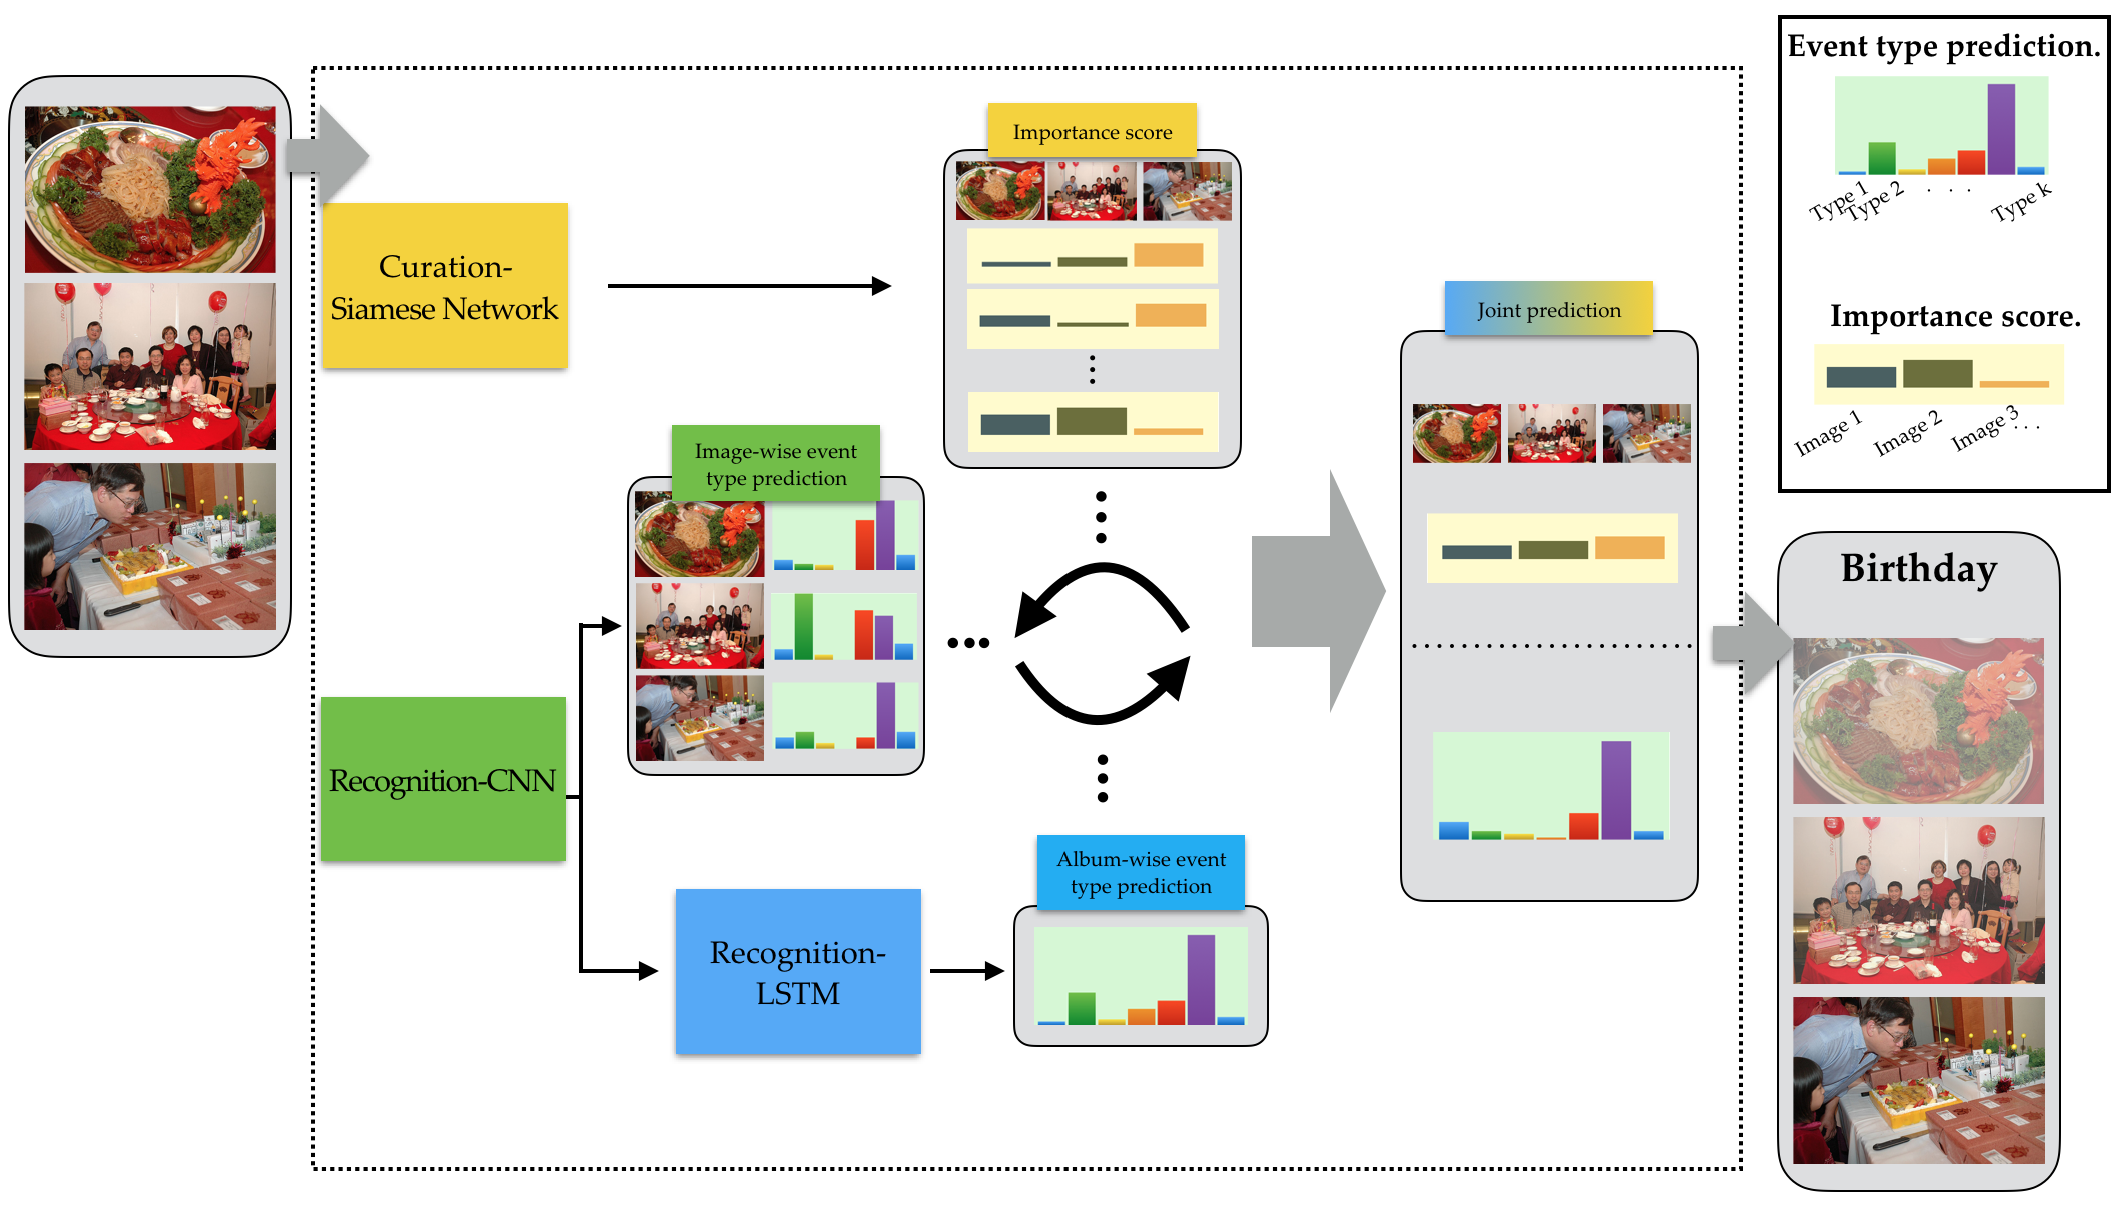
\includegraphics[width=4.8in]{architecture}
\caption{The joint album recognition-curation system. The system consists of three parts: a Siamese network for image importance score prediction, a CNN for single image event-type recognition, and an LSTM network for album-wise event-type recognition. During the test stage, followed by a iterative updating rule, the three components interact and jointly produce the prediction of album event type and image importance score. }
\label{figure1}
\vspace{-0.3in}
\end{figure}

\subsection{Event curation network}
\label{curation_section}
%\textcolor{red}{Not sure how detailed should  the part of previous paper be.}

For event curation purposes, we followed the approach in \cite{CVPR}, using Piecewise Ranking (PR) loss to jointly train a Siamese network to predict the importance score difference between an image pair given the ground-truth event type of the input image pair. The architecture can predict the relative event-specific importance score for a set of images, and is found to perform better than a traditional CNN that directly predicts the absolute important score of an image.
One difference in our implementation compared to \cite{CVPR} is that the ground-truth event for the input image pair  is not a one-hot representation; instead, it is represented as a probability distribution. In \cite{CVPR}, the event type label is used to gate the output and the gradient of the Siamese network: for an input image pair of a certain event type $c \in C$, only the part of the network which corresponds to event type $c$ is back-propagated.  Here, to train the Siamese network on the multi-event type label, we change the 0/1 gating to a soft gating, thus for an input image pair with multiple event type labels, the error signals from all the possible labels are back-propagated, but with a weight: the ground-truth probability of that event type. Another scheme is to use 0/1 gating, but for an input image pair with multiple event type labels, it assumes equal probability for the network to treat the input image pair as from one of the possible labels. This gives more relaxation on the ground-truth event type label.
% * <gary@ucsd.edu> 2016-03-15T04:27:49.346Z:
%
% > only the part of the network which corresponds to event type $c$ is back-propagated.
%
% I'm not clear what that means. You back propagate to the whole network, it is just through the weights to the event type, right?
%
% ^ <gary@ucsd.edu> 2016-03-15T04:29:47.558Z:
%
% I mean, you can simply say you back-propagated through the event node, like a max-pooling unit.
%
% ^.
\subsection{Event recognition network}
One of the properties of  an ``event album" that makes it different from a simple collection of images is that it is a sequence, and this provides us with the temporal relationship between the images. LSTMs have been successfully applied to sequential tasks, and its ability to do long-range context memorization is suitable for our task of album-wise event recognition. Therefore, we use the LSTM network to capture the sequential information, in addition to a classical CNN that captures the visual features of a single image. 

We start with a CNN pre-trained on ImageNet \cite{caffe} \cite{imagenet}, and fine-tune it on the ML-CUFED Dataset to recognize a single image's event type. We then extract the high level CNN features for each image from the adapted network, and use them as the input features to train the LSTM network for album-wise event recognition. The LSTM network consists of a single LSTM layer, a mean pooling layer, and a softmax prediction layer. 


The target for both the fine-tuned CNN and LSTM network is the soft distribution of the ground-truth event labels. Again, another scheme is to use the one-hot target, but treat each training example as from one of the possible event types with equal probabilities. 
% * <gary@ucsd.edu> 2016-03-15T04:33:08.745Z:
%
% > with equal probabilities. 
%
% why with equal probabilities? Why not according to the distribution of labels?
%
% ^.

During testing stage, the prediction of an album type is achieved by simply averaging the two predictions from CNN and LSTM.




\subsection{The iterative curation-recognition procedure}
For an ``event album", more interesting images or important images give us more information about the event type of this album. For example, although a candle blowing image may only appear in an album once, it is very helpful for deciding the event type of the album. However, as shown in \cite{CVPR}, the importance of an image is related to the context it is in, and is event-type dependent. Therefore, we propose that the image importance score can help with event recognition of an album, while event recognition of an album will in turn improve the image importance score prediction.

We denote an $N$-image album as $\mathbf{A}= \left \{I^{1}, ..., I^{N}  \right \}$. The output of the algorithm is the $N$-dimensional column vector $V = [v^{1}, ..., v^{N}]^{T}$, which is the prediction for all images' importance score in album $\mathbf{A}$, and the $C$-dimensional column vector $P = [p_{1}, p_{2},..., p_{C}]^{T}$ is the prediction for the album's event type. Here, $C$ is the number of event types. 


We also need to define the intermediate result we need to perform the iterative update. From the event curation Siamese Network in Section~\ref{curation_section}, we obtain the importance score of an image $I^{n} \in \mathbf{A} $ given its event type: $W^{n}= \left [w_{1}^{n} , ..., w_{C}^{n}  \right ]^{T}$
From the event recognition CNN, we can get the estimated probability distribution of the event type for a single image
$Q^{n}= \left [ q_{1}^{n} , ..., q_{C}^{n}  \right ]^{T}$. Moreover, from the LSTM network, we can get the estimated probability distribution of the event type for the album $\hat{P} = [\hat{p}_{1}, ..., \hat{p}_{C}]^{T}$. 


The iterative curation-recognition procedure can be described as follows:
\begin{enumerate}
  \item \textbf{Update album event type prediction} from the CNN with predicted image importance score $V(k)$.
  \begin{equation}
  \check{p}_{c}(k+1) = V^{T}(k)^{\alpha }\cdot  Q^{n}
  \label{eq1}
  \end{equation}
  where the $N$-dimensional column vector $V(k) = [v^{1}, ..., v^{N}]^{T}$ is the $k$-th step prediction for all images' importance score in album $A$ (initialized to a uniform distribution). $\check{P} = [\check{p}_{1}, ... \check{p}_{C}]$ denotes the updated  album event type prediction. Thus, the (k+1)-step album-wise prediction of the event type is the average of each image's prediction weighted by the image's predicted importance score. $\alpha$ controls the strength importance score has for the update.
% * <gary@ucsd.edu> 2016-03-15T05:33:38.013Z:
%
% > Here, $V$ is initialized to a uniform distribution.
%
% I don't understand why V isn't initialized to W.
%
% ^.
% * <gary@ucsd.edu> 2016-03-15T04:59:34.272Z:
%
% > $\check{P} = [\check{p}_{1}, ... \check{p}_{C}]$ denotes the album event type prediction from the CNN.
%
% You have already defined the CNN prediction as Q, right? So this must be the *updated* event type distribution.
%
% ^.
\vspace{0.05in}
    \item \textbf{Combine event type predictions} with $\hat{P}$.
  \begin{equation}
  p_{c}(k+1) = \frac{1}{2}(\check{p}_{c}(k+1) + \hat{p}_{c})
  \label{eq2}
  \end{equation}
Thus, the prediction of LSTM network is averaged with the weighted event type from step 1 to update the event type prediction. $p_{c}$ is then renormalized. 
% * <gary@ucsd.edu> 2016-03-15T05:33:19.099Z:
%
% ^.
\vspace{0.05in}
  \item \textbf{Update image importance score prediction} with the event type prediction $P(k+1)$.
  \begin{equation}
v^{n}(k+1) = \left \{W_{n}^{T} \circ \textup{I}\left \{ p^{n}_{c}\geq m\cdot \max_{c'}(p^{n}_{c'}) \right \}_{(c,1)}\right \} \cdot  P(k+1)
  \label{eq3}
\end{equation}
 where $\circ$ denotes element-wise matrix multiplication and \textup{I} is an indicator function that returns 1 if its argument is true and 0 otherwise. Thus, the update image importance is acquired from the average of the importance score given different event types, weighted by the event type probability. The argument to \textup{I} computes whether $p^{n}_{c}$ is larger than a fraction $m$ (a parameter) of the maximum probability, so creates a binary mask that eliminates the event type predictions with low confidence. 
% * <gary@ucsd.edu> 2016-03-15T05:02:30.925Z:
%
% > denotes the binary mask that eliminates the event type predictions with low confidence, and makes sure only event types with high probability contribute to the image importance update. 
%
% is this necessary? If they have low probability, won't they contribute very little anyway?
%
% ^ <gary@ucsd.edu> 2016-03-15T05:04:32.808Z:
%
% So, m denotes a fraction of the maximum event type probability?
%
% ^.
\end{enumerate}

By iterating Equations~\ref{eq1}-\ref{eq3}, we obtain the album-wise event prediction $P$ and image importance score prediction $V$. 

Note that this procedure is not guaranteed to converge, hence we set a maximum number of iterations, and if this maximum number is reached, the predictions for $Q$ and $V$ are obtained by averaging over the three previous steps.

The entire system is illustrated in Figure~\ref{figure1}.

\section{Experiments}
In this section, we evaluate our approach for both event recognition and image importance prediction on the ML-CUFED Dataset, and we compare our event recognition result with \cite{HMM} on the PEC Dataset.
\subsection{Baselines}
Our joint recognition-curation method produces two outputs: album event type prediction, and image event-importance prediction. 
For event recognition, we compare our result with the baseline by training a single CNN to classify each input image into event types. We denote this method CNN-recognition. In addition, the intermediate result of our algorithm can also be compared with the final result to validate the necessity of each part of our system. Therefore, we compare our method with the following methods:
\begin{itemize}
  \item \textbf{CNN-recognition}: Use a single CNN to predict the event type for a single image. To predict the event type of one album, predictions of all the images are averaged.
  \item \textbf{CNN-Iterative}: Use the event type prediction from the CNN-recognition network and the image importance prediction result from the Siamese Network to jointly obtain the modified recognition prediction. Here, no LSTM network result is involved. 
    \item \textbf{CNN-LSTM}: Use the feature extracted from CNN-recognition as input to an LSTM network, and directly predict the album event type given the input image sequence.
  \item \textbf{CNN-LSTM-Iterative}: proposed method as described in Section~\ref{approach}, using CNN-recognition and LSTM to predict the event type label, the Siamese network to predict the importance of images, and use iterative update rule to obtain the final prediction for the album-wise event type prediction. 
\end{itemize}

To evaluate our image importance prediction result, we provide a comparison with several baselines:
\begin{itemize}
  \item \textbf{CNN-Noevent}: Train a Siamese Network to predict the importance score difference of an input image pair. No event type information is given to the network while training or testing. All albums are considered having the same ``hyper" event type.
  \item \textbf{CNN-Noevent(test)}: When training the Siamese Network, use the ground-truth event type information to gate the output error and back-propagation signal. In this way, features for each event type are learned separately. When testing, given an image, average the predicted importance score for all possible event types.  
    \item \textbf{CNN-LSTM-Iterative}: As above.
    \end{itemize}

\subsection{Experimental Details}
\paragraph{Dataset} For ML-CUFED Dataset, we split the albums to training:test 4:1. The test set has 368 albums. To decide the hyper-parameters $(\alpha, m)$ in our iterative model, a validation set with 119 albums is separated from the training set.  For the PEC Event Recognition Dataset \cite{HMM}, we use directly the test set consisting of 10 albums for each event type as described in \cite{HMM}, so that we can directly compare it with our methods.

\paragraph{Parameter setting} For both the CNN-recognition network and the Siamese network, we use the 8-layer AlexNet \cite{imagenet} pretrained on ImageNet as the starting point, and fine-tune it on the ML-CUFED Dataset. We use a similar training scheme to \cite{caffe}, but with a lower learning rate of 0.001. For the LSTM network, we use the 7th layer feature from the trained CNN-recognition as the input. The 7th layer feature is 4096-dimensional, and we reduce it to 128-dimensional with PCA. For the LSTM network, we use AdaDalta as optimization method \cite{adadelta,theano1,theano2}. For the Siamese network, we follow the settings in \cite{CVPR} and choose the two thresholds as $m_{s} = 0.1$ and $m_{d}=0.3$. We set the nubmer of iteration of our joint recognition curation algorithm to 10.

\paragraph{Evaluation} For event recognition, we use two metrics to evaluate different methods: average accuracy and $\textup{F}_{1}$ Score.  $\textup{F}_{1}$ Score is the harmonic mean of precision and recall, and can account for multi-label groundtruth. For ML-CUFED where multi-label ground-truth is allowed, both accuracy and $\textup{F}_{1}$ are calculated with top-1 prediction. For image importance prediction, we follow the evaluation metrics in \cite{CVPR}, using MAP@($t\%$) and Precision P@($t\%$).  Precision is calculated as the ratio between the number of retrieved relevant images and the number of all relevant images. MAP is the averaged area under the precision-recall curve, and can be calculated:
\begin{equation}
\textup{AP(S)}@t\%=\int_{0}^{1}p(r)d(r)\approx \frac{\sum_{k=1}^{n}p(k)\times \textup{rel}(k)}{\left \lceil n\cdot t\% \right \rceil}
\end{equation}
\begin{equation}
\textup{MAP(U)}@t\% = \frac{1}{N}\sum_{i=1}^{N}\textup{AP}(\textup{A}_{i})@t\%
\end{equation}




\subsection{Results on the ML-CUFED Dataset}
\subsubsection{Event-specific image importance}

For the event-specific image importance score prediction task, we provide the comparison of our methods with several baselines in Table~\ref{aesthetic_table}. To show the upper-bound of our method, we also show the result for CNN-Cheating: where we assume the ground truth even type is known for each test album,  and use the predicted importance score for that ground-truth event type as the final importance prediction. Note that in our setting we assume only albums are given, and no additional information is added. Therefore, the result of CNN-Cheating here just serves as the best result we can get when the event recognition stage is perfect. The CNN-Cheating result is very similar to that achieved in \cite{CVPR}. As shown in Table~\ref{aesthetic_table}, CNN-Noevent performs a little better than CNN-Noevent (test). This suggests the divergence of the importance prediction for different event types. CNN-Iterative outperforms CNN-Noevent greatly, with a steady 3\% MAP increment. There is also a steady 3\% increment for $\textup{P}$ at $t<20\%$.

CNN-Iterative greatly reduces the performance loss from knowing the event types (CNN-Cheating) to not knowing the event types (CNN-Noevent), and approaches closely the upper bound (CNN-Cheating).
\begin{table}[]
\centering
\scalebox{0.9}{
\begin{tabular}{c|cccccc|cccccc}
\thickhline
          & \multicolumn{6}{c|}{$\mathbf{MAP}@\mathbf{t\%}$}          & \multicolumn{6}{c}{$\mathbf{P}@\mathbf{t\%}$} \\ \thickhline
t\%       & 5     & 10    & 15    & 20    & 25    & 30    & 5  & 10  & 15 & 20 & 25 & 30 \\ \hline
Random & 0.113 & 0.161 & 0.211 & 0.256 & 0.303 & 0.350 & 0.044  &  0.090   &  0.142  &  0.193  & 0.243   & 0.298   \\
CNN-Noevent(test) & 0.251 & 0.303 & 0.358 & 0.414 & 0.462 & 0.508 & 0.142   &  0.211   & 0.284   & 0.335   &   0.384 & 0.436    \\
CNN-Noevent & 0.258 & 0.316 & 0.369 & 0.425 & 0.475 & 0.519  & 0.168   &  0.245   & 0.307   & 0.373   &   0.422 & 0.468 \\ 
CNN-Iterative &0.278&0.347&0.400&0.453&0.502&0.547&0.191&0.280&0.340&0.394&0.450&0.491 \\ \hline
CNN-Cheating &0.305&0.372&0.424&0.476&0.522&0.565&0.218&0.304&0.361&0.417&0.461&0.504 \\ 
\thickhline
\end{tabular}
}
\caption{Comparison of event-specific image importance predictions using different methods. Evaluation metric here is $\text{MAP}@t\%$ and $P@t\%$. We also show Random ranking score as a lower bound. We also provide a CNN-cheating result which uses ground-truth event type information when testing as an upper-bound.}
\label{aesthetic_table}
\vspace{-0.35in}
\end{table}



\subsubsection{Event recognition}
Table~\ref{CUFED} shows the results of different methods for event recognition. Note that ML-CUFED allows multiple labels, therefore the accuracy here is different from the conventional accuracy: for an album, we only evaluate the top 1 prediction. If the predicted event type is among the ground-truth event labels, we deem this album correctly predicted.
As shown, there is more than 4\% performance gain on the average accuracy, and 4\% gain on $F_{1}$ Score, from the baseline CNN-recognition method to our proposed method. We can also observe that both iterative curation-recognition and LSTM method help to improve the final result. This suggests that both these types of information in an event album are helpful in deciding the event type of this album: image importance information, and album sequential information. 

\begin{table}[]
\vspace{-0.2in}
\centering
\scalebox{0.9}{
\begin{tabular}{cccc}
\thickhline
\textbf{Method}             & \textbf{Avg. Acc. } & \textbf{$\mathbf{F}_{1}$-Score} \\ \hline
CNN-recognition    & 75.0\%        &   0.698       \\
CNN-Iterative      & 78.0\%         &   0.729       \\
CNN-LSTM               & 76.6\%              &   0.713  \\
CNN-LSTM-Iterative & 79.1\%      &       0.737      \\ \thickhline
\end{tabular}
}
\caption{Comparison of different event-recognition methods on ML-CUFED Dataset.}
\label{CUFED}
\vspace{-0.4in}
\end{table}



Figure~\ref{confusion} provides the confusion matrix of the baseline CNN-recognition and proposed method CNN-LSTM-Iterative. To allow for multi-label, each pair of (ground truth label, prediction) counts for one point in the confusion matrix.
We can observe an overall performance gain from the baseline method to CNN-LSTM-Iterative, and an overall reduction of confusions from baseline to proposed method. Note, though, there are two categories with 0\% accuracy: Personal Art Activity, and Personal Musical Activity. This is caused by the intrinsic high ambiguity and lack of training data for these two event types (there are only 23 albums with Personal Music Activity in the entire dataset, and all of them have multiple votes). 


In Figure~\ref{resultcufed}, we show our event curation and recognition result with two examples in the ML-CUFED Dataset. The image are ranked in ground-truth importance order, and the predicted importance score is labeled below the image. More examples are presented in the supplementary material. 
\begin{figure}
\vspace{-0.25in}
\centering
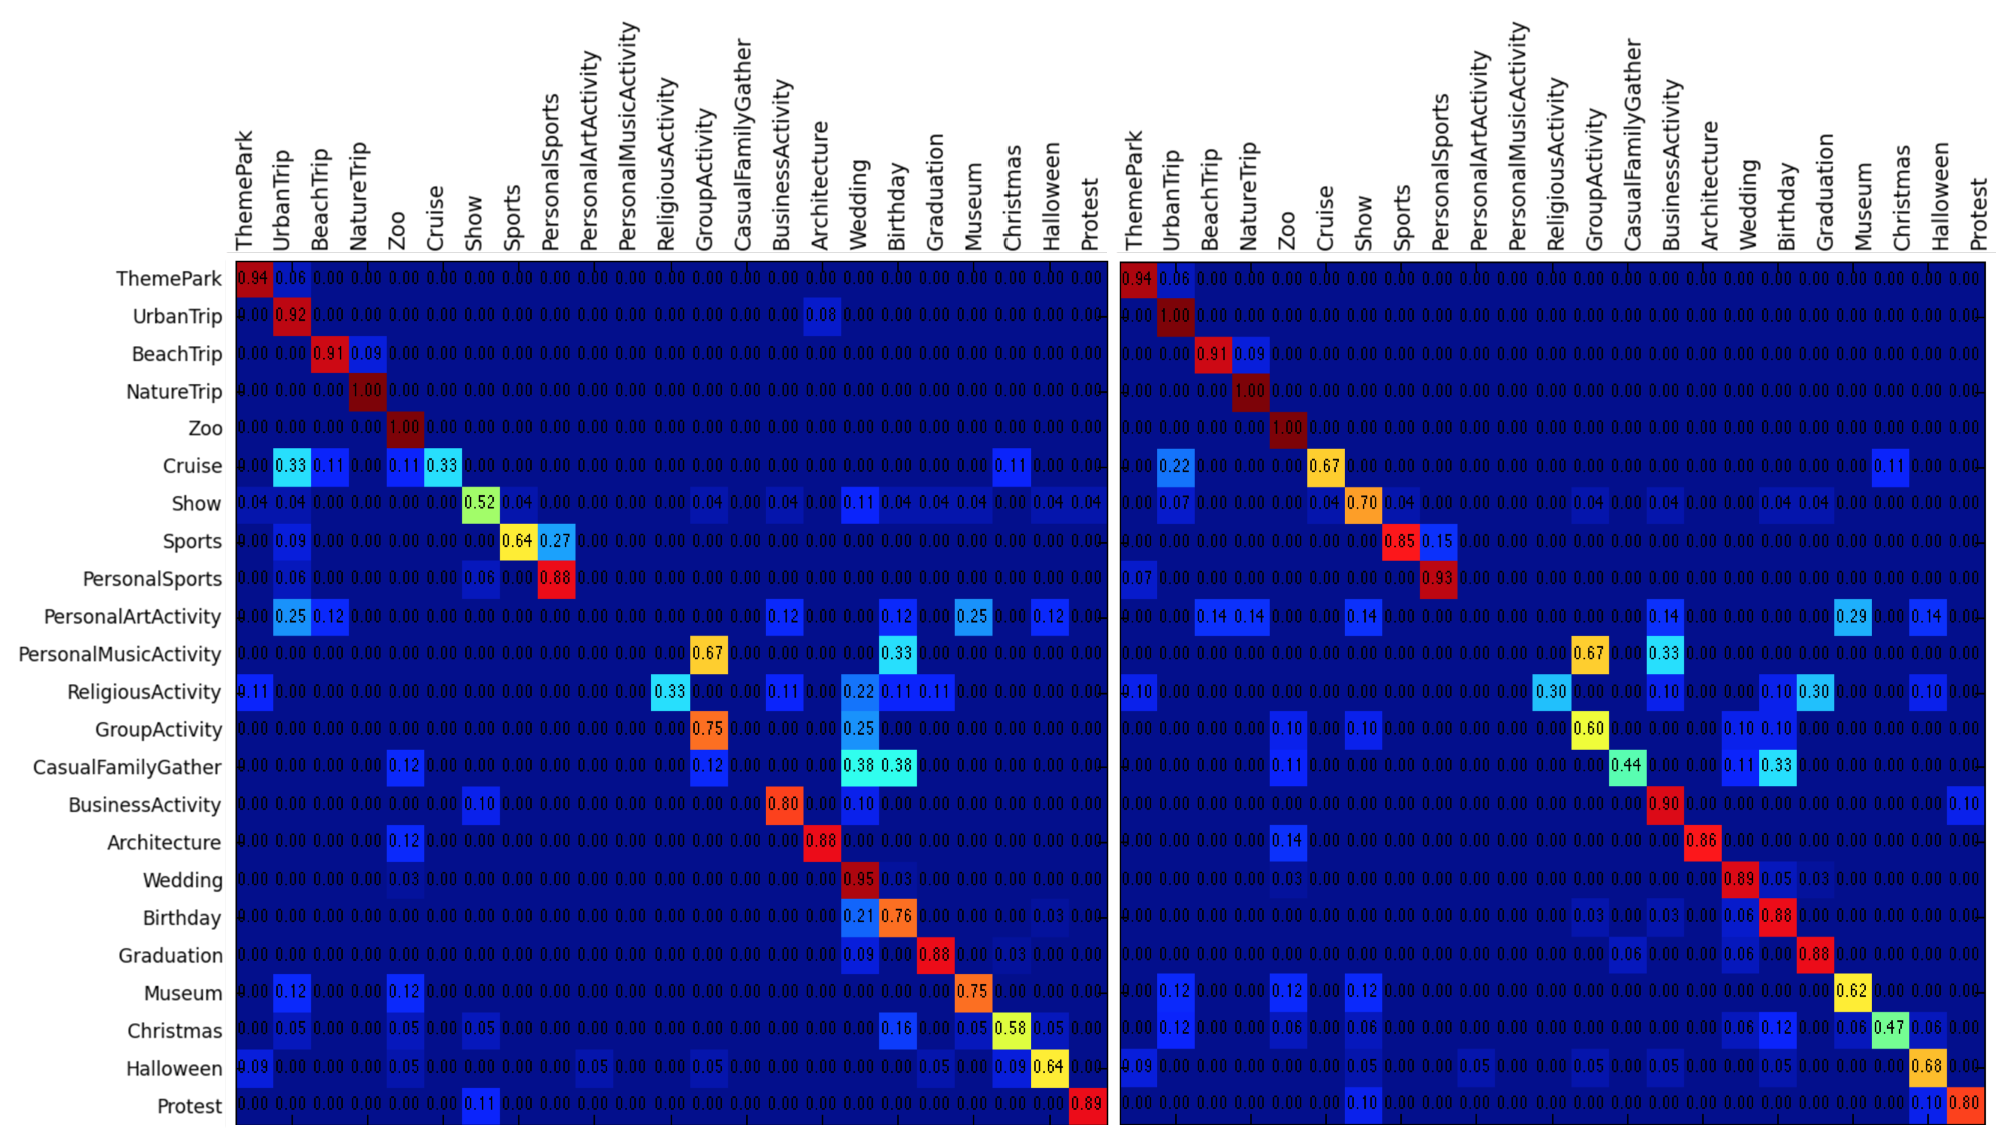
\includegraphics[width=3.5in]{confusion_new}
\caption{Confusion matrices for the baseline method(left) and our proposed method CNN-LSTM-Interative (right).}
\label{confusion}
\vspace{-0.3in}
\end{figure}

\begin{figure}
\vspace{-0.15in}
\centering
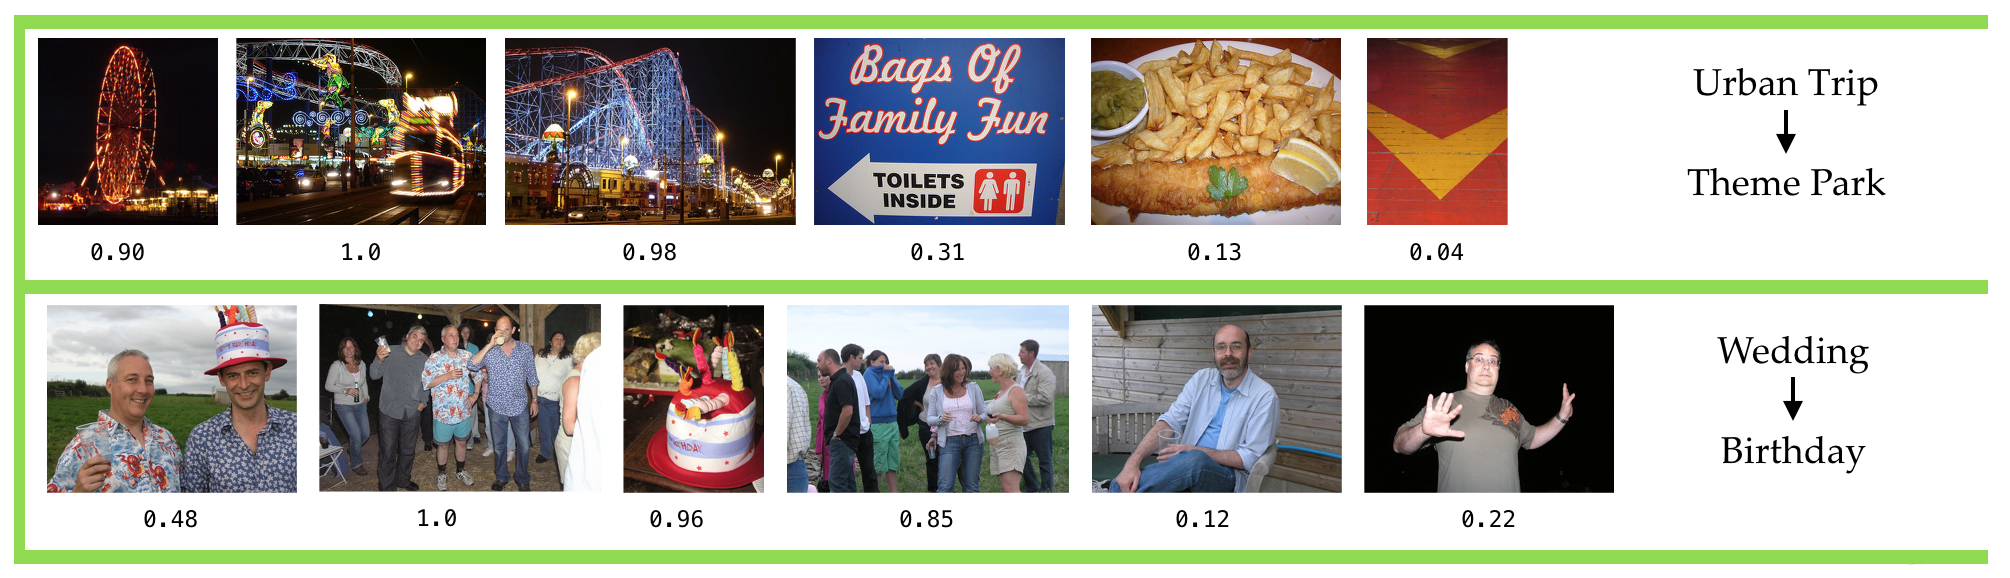
\includegraphics[width=3.5in]{result-cufed}
\caption{Examples of recognition-curation result from ML-CUFED Dataset.}
\label{resultcufed}
\vspace{-0.28in}
\end{figure}


\subsection{Results on the PEC Dataset}
\label{PEC_section}
To show the generalizability of our algorithm, we compare our result with \cite{HMM} on their PEC Dataset.

The PEC Dataset is an 807-album event dataset, with 14 social event classes. There is no ground-truth importance score labels in PEC, thus we cannot train our algorithm on it. Therefore, we use the model we trained on ML-CUFED and test the model on the PEC test set containing 10 albums each class, and compare with the result achieved in \cite{HMM} to make a fair comparison.

In the PEC Dataset, there are several event types that are not contained in ML-CUFED, such as Saint Patrick's Day, Easter, and Skiing, and there are multiple event types that can map to single event type in ML-CUFED: Children's Birthday and Birthday can be mapped to single Birthday event in the ML-CUFED dataset. Therefore, we provide the mapping from PEC label to ML-CUFED label in Table~\ref{table1}. Note that the mapping is not perfect. For example, although most albums in Road Trip(PEC) fall into Nature Trip(ML-CU), some of them should fall into Urban Trip(ML-CU), but our mapping ignore this to avoid any bias it might bring to the evaluation. The noise in the mapping makes the performance of our method shown here a little poorer than it really is.

Due to the label changes, we recalculate the performance of Stopwatch HMM (SHMM) \cite{HMM} on the test data. Merged labels are straightforward to deal with, just by merging the two corresponding rows in the confusion matrix. However, for missing labels, there are three possible approaches: 1. Assume false positive on those labels will be correct predictions if those labels disappear; 2. Assume false positive on those labels will still be incorrect; 3 Ignore false positive on those labels, shrinking the size of the test set. 1 and 2 are two extreme ends, being very loose and very strict respectively, while 3 lies in the middle. 

It is also easy to calculate the accuracy of our model: We still take the maximum of predicted probabilities from our model, but ignore those that don't belong in Table~\ref{table1}.

The comparison of different methods is shown in Table~\ref{PEC}. For the result of SHMM, we provide all the three criteria mentioned above. It is worth noting that our networks are fully trained on ML-CUFED, and despite the difference between the two datasets (collected from different sources) and the inevitable label mis-matching, even our baseline method (CNN-recognition)  outperforms SHMM. Similar to the result on ML-CUFED, we observe a performance gain from both LSTM network and iterative updates.

\begin{table}[]
\vspace{-0.1in}
\small
\centering
\scalebox{0.9}{
\begin{tabular}{c|c|c|c|cc}
 \thickhline
\textbf{PEC}      & (Children's) Birthday  & Christmas         & Concert & \multicolumn{1}{c|}{Cruise} & Exhibition \\  
\textbf{ML-CUFED} & Birthday                      & Christmas         & Show    & \multicolumn{1}{c|}{Cruise} & Museum     \\ \hline
\textbf{PEC}      & Halloween                     & Hiking, Road Trip & Wedding & Graduation                  &            \\
\textbf{ML-CUFED} & Halloween                     & Nature Trip       & Wedding & Graduation                  &           \\ \thickhline
\end{tabular}
}
\caption{Event type matching from PEC Dataset to ML-CUFED Dataset.}
\label{table1}
\end{table}
\vspace{-0.6in}

\begin{table}[]
\centering
\scalebox{0.9}{
\begin{tabular}{ccc}
\thickhline
\textbf{Method}             & \textbf{Avg. Acc.} & \textbf{$F_{1}$-Score} \\ \hline
SHMM               & 76.3(1) / 59.1(2) / 72.2(3)\% &  -\\
CNN-recognition    & 80.9\%        &   0.805          \\
CNN-Iterative      & 81.8\%        &   0.810       \\
CNN-LSTM               & 82.7\%              &   0.824  \\
CNN-LSTM-Iterative & 84.5\%      &       0.842      \\ \thickhline
\end{tabular}
}
\caption{Comparison of different methods on PEC Dataset. For the SHMM result, accuracies under three criteria are provided. See Section~\ref{PEC_section} for details.}
\label{PEC}
\vspace{-0.4in}
\end{table}

We show some of the examples of our recognition and event-specific image importance prediction result in Figure~\ref{pec_result}. Although there is no ground-truth labeling for the event-specific importance score for the images, we can look at the sample results qualitatively. From the first row in Figure~\ref{pec_result}, we can see that the model does not simply assign a high importance score to the characteristic Christmas tree, but predicts a very high score when there are people sitting in front of the Christmas tree. From the second row, we can see the property of the event modulated importance score: although the first image of the beautiful architecture should have a high importance in a trip album, in the birthday album, it is much less important even than the image of the table of celebrative food.
\begin{figure}[ht]
\centering
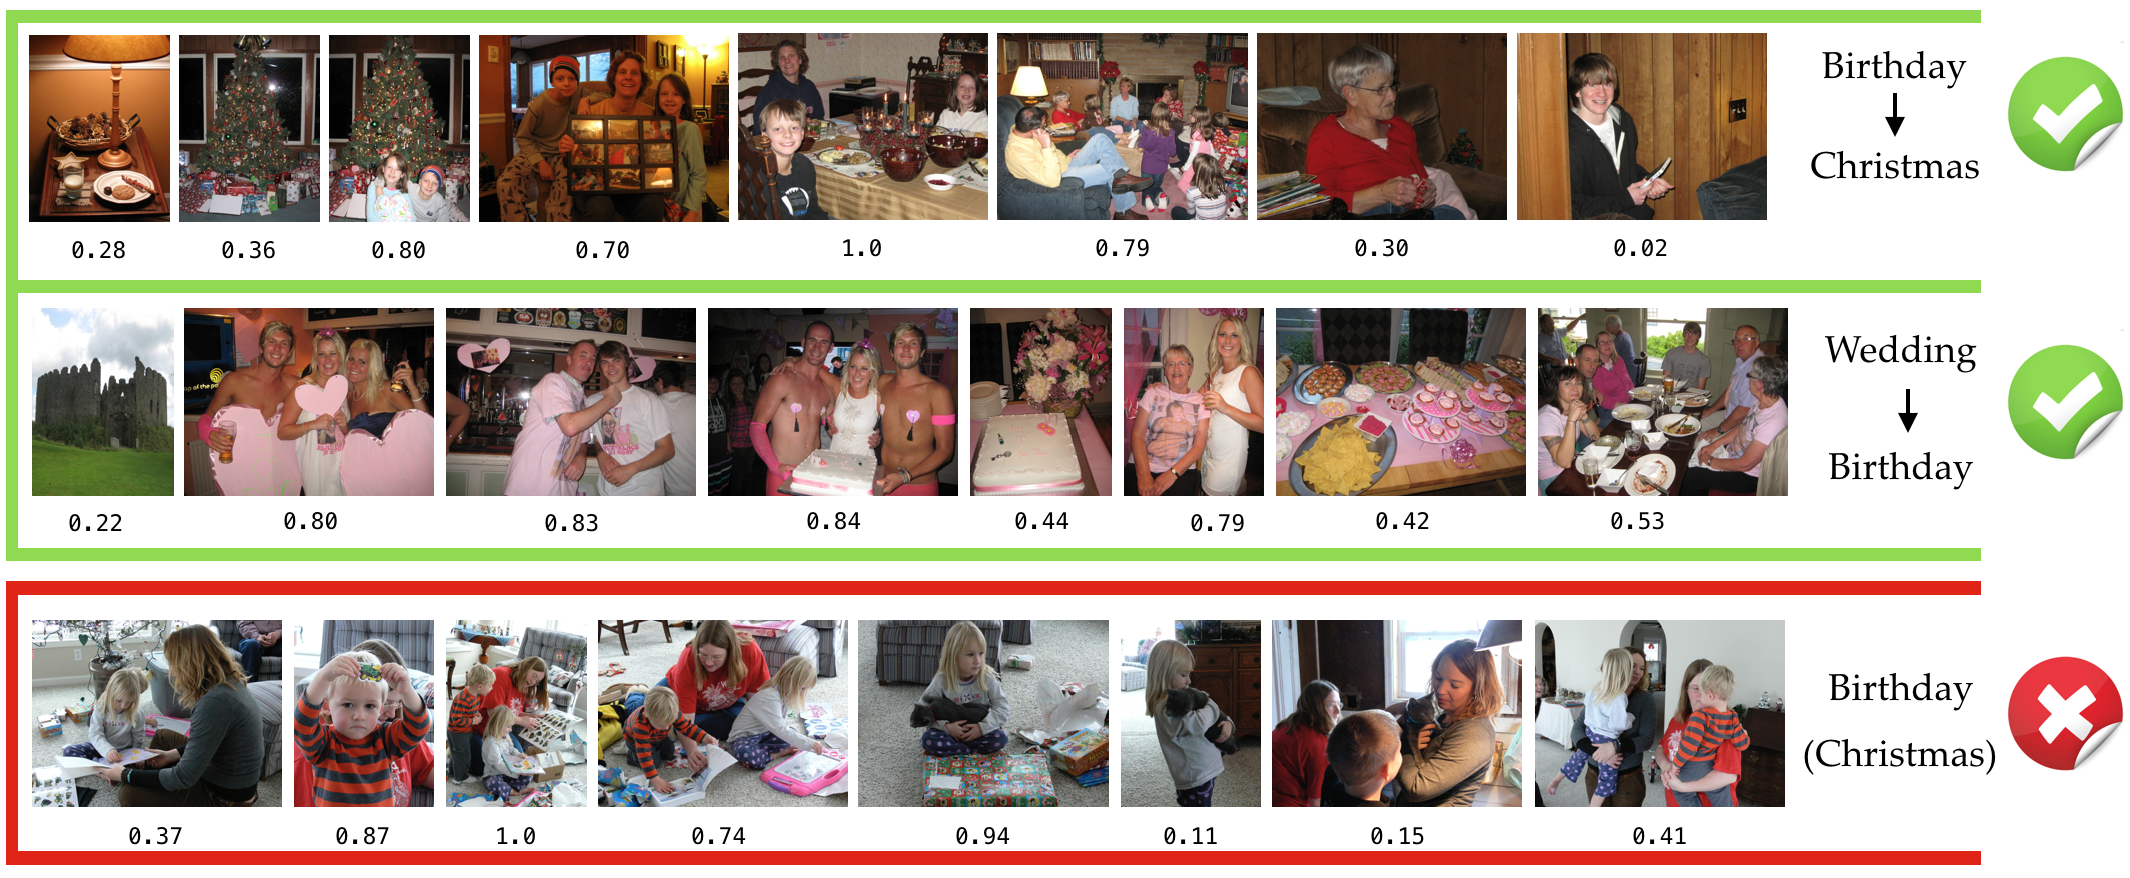
\includegraphics[width=4.8in]{pec_result}
\caption{Some results from the PEC Dataset. For first two rows, the prediction from CNN-Direct is wrong as shown in the label above, whereas the sequential information helps the algorithm to modify the final prediction to give the correct answer. For the third row, a case where the model fails to recognize a Christmas event is shown. The predicted importance score of each image is shown below the corresponding image. Only a subset of images is shown here for each album due to limited space.}
\label{pec_result}
\vspace{-0.15in}
\end{figure}

\section{Conclusion}
In this work, we explore into the problem of organizing personal photo collections. This work is the first attempt to solve simultaneously the following problems: recognizing the event type of an album, and finding the important images in the album corresponding to the event type. We develop a joint algorithm for the task: the result from a CNN for image-wise event recognition, an LSTM Network for album-wise event recognition, and a Siamese Network for image importance prediction are merged by an iterated updating algorithm. We show that the joint algorithm improves both image importance recognition and event recognition. This suggests that image importance and sequential information are helpful for album-wise event recognition, and that the event recognition result can in turn help with better image selection. 
\clearpage



\clearpage
\bibliographystyle{splncs}
\bibliography{egbib}
\end{document}

